%% bare_jrnl.tex
%% V1.4b
%% 2015/08/26
%% by Michael Shell
%% see http://www.michaelshell.org/
%% for current contact information.
%%
%% This is a skeleton file demonstrating the use of IEEEtran.cls
%% (requires IEEEtran.cls version 1.8b or later) with an IEEE
%% journal paper.
%%
%% Support sites:
%% http://www.michaelshell.org/tex/ieeetran/
%% http://www.ctan.org/pkg/ieeetran
%% and
%% http://www.ieee.org/

%%*************************************************************************
%% Legal Notice:
%% This code is offered as-is without any warranty either expressed or
%% implied; without even the implied warranty of MERCHANTABILITY or
%% FITNESS FOR A PARTICULAR PURPOSE! 
%% User assumes all risk.
%% In no event shall the IEEE or any contributor to this code be liable for
%% any damages or losses, including, but not limited to, incidental,
%% consequential, or any other damages, resulting from the use or misuse
%% of any information contained here.
%%
%% All comments are the opinions of their respective authors and are not
%% necessarily endorsed by the IEEE.
%%
%% This work is distributed under the LaTeX Project Public License (LPPL)
%% ( http://www.latex-project.org/ ) version 1.3, and may be freely used,
%% distributed and modified. A copy of the LPPL, version 1.3, is included
%% in the base LaTeX documentation of all distributions of LaTeX released
%% 2003/12/01 or later.
%% Retain all contribution notices and credits.
%% ** Modified files should be clearly indicated as such, including  **
%% ** renaming them and changing author support contact information. **
%%*************************************************************************


% *** Authors should verify (and, if needed, correct) their LaTeX system  ***
% *** with the testflow diagnostic prior to trusting their LaTeX platform ***
% *** with production work. The IEEE's font choices and paper sizes can   ***
% *** trigger bugs that do not appear when using other class files.       ***                          ***
% The testflow support page is at:
% http://www.michaelshell.org/tex/testflow/



\documentclass[journal]{IEEEtran}
%
% If IEEEtran.cls has not been installed into the LaTeX system files,
% manually specify the path to it like:
% \documentclass[journal]{../sty/IEEEtran}





% Some very useful LaTeX packages include:
% (uncomment the ones you want to load)


% *** MISC UTILITY PACKAGES ***
%
%\usepackage{ifpdf}
% Heiko Oberdiek's ifpdf.sty is very useful if you need conditional
% compilation based on whether the output is pdf or dvi.
% usage:
% \ifpdf
%   % pdf code
% \else
%   % dvi code
% \fi
% The latest version of ifpdf.sty can be obtained from:
% http://www.ctan.org/pkg/ifpdf
% Also, note that IEEEtran.cls V1.7 and later provides a builtin
% \ifCLASSINFOpdf conditional that works the same way.
% When switching from latex to pdflatex and vice-versa, the compiler may
% have to be run twice to clear warning/error messages.






% *** CITATION PACKAGES ***
%
%\usepackage{cite}
% cite.sty was written by Donald Arseneau
% V1.6 and later of IEEEtran pre-defines the format of the cite.sty package
% \cite{} output to follow that of the IEEE. Loading the cite package will
% result in citation numbers being automatically sorted and properly
% "compressed/ranged". e.g., [1], [9], [2], [7], [5], [6] without using
% cite.sty will become [1], [2], [5]--[7], [9] using cite.sty. cite.sty's
% \cite will automatically add leading space, if needed. Use cite.sty's
% noadjust option (cite.sty V3.8 and later) if you want to turn this off
% such as if a citation ever needs to be enclosed in parenthesis.
% cite.sty is already installed on most LaTeX systems. Be sure and use
% version 5.0 (2009-03-20) and later if using hyperref.sty.
% The latest version can be obtained at:
% http://www.ctan.org/pkg/cite
% The documentation is contained in the cite.sty file itself.






% *** GRAPHICS RELATED PACKAGES ***
%
\ifCLASSINFOpdf
  % \usepackage[pdftex]{graphicx}
  % declare the path(s) where your graphic files are
  % \graphicspath{{../pdf/}{../jpeg/}}
  % and their extensions so you won't have to specify these with
  % every instance of \includegraphics
  % \DeclareGraphicsExtensions{.pdf,.jpeg,.png}
\else
  % or other class option (dvipsone, dvipdf, if not using dvips). graphicx
  % will default to the driver specified in the system graphics.cfg if no
  % driver is specified.
  % \usepackage[dvips]{graphicx}
  % declare the path(s) where your graphic files are
  % \graphicspath{{../eps/}}
  % and their extensions so you won't have to specify these with
  % every instance of \includegraphics
  % \DeclareGraphicsExtensions{.eps}
\fi
% graphicx was written by David Carlisle and Sebastian Rahtz. It is
% required if you want graphics, photos, etc. graphicx.sty is already
% installed on most LaTeX systems. The latest version and documentation
% can be obtained at: 
% http://www.ctan.org/pkg/graphicx
% Another good source of documentation is "Using Imported Graphics in
% LaTeX2e" by Keith Reckdahl which can be found at:
% http://www.ctan.org/pkg/epslatex
%
% latex, and pdflatex in dvi mode, support graphics in encapsulated
% postscript (.eps) format. pdflatex in pdf mode supports graphics
% in .pdf, .jpeg, .png and .mps (metapost) formats. Users should ensure
% that all non-photo figures use a vector format (.eps, .pdf, .mps) and
% not a bitmapped formats (.jpeg, .png). The IEEE frowns on bitmapped formats
% which can result in "jaggedy"/blurry rendering of lines and letters as
% well as large increases in file sizes.
%
% You can find documentation about the pdfTeX application at:
% http://www.tug.org/applications/pdftex





% *** MATH PACKAGES ***
%
%\usepackage{amsmath}
% A popular package from the American Mathematical Society that provides
% many useful and powerful commands for dealing with mathematics.
%
% Note that the amsmath package sets \interdisplaylinepenalty to 10000
% thus preventing page breaks from occurring within multiline equations. Use:
%\interdisplaylinepenalty=2500
% after loading amsmath to restore such page breaks as IEEEtran.cls normally
% does. amsmath.sty is already installed on most LaTeX systems. The latest
% version and documentation can be obtained at:
% http://www.ctan.org/pkg/amsmath





% *** SPECIALIZED LIST PACKAGES ***
%
%\usepackage{algorithmic}
% algorithmic.sty was written by Peter Williams and Rogerio Brito.
% This package provides an algorithmic environment fo describing algorithms.
% You can use the algorithmic environment in-text or within a figure
% environment to provide for a floating algorithm. Do NOT use the algorithm
% floating environment provided by algorithm.sty (by the same authors) or
% algorithm2e.sty (by Christophe Fiorio) as the IEEE does not use dedicated
% algorithm float types and packages that provide these will not provide
% correct IEEE style captions. The latest version and documentation of
% algorithmic.sty can be obtained at:
% http://www.ctan.org/pkg/algorithms
% Also of interest may be the (relatively newer and more customizable)
% algorithmicx.sty package by Szasz Janos:
% http://www.ctan.org/pkg/algorithmicx




% *** ALIGNMENT PACKAGES ***
%
%\usepackage{array}
% Frank Mittelbach's and David Carlisle's array.sty patches and improves
% the standard LaTeX2e array and tabular environments to provide better
% appearance and additional user controls. As the default LaTeX2e table
% generation code is lacking to the point of almost being broken with
% respect to the quality of the end results, all users are strongly
% advised to use an enhanced (at the very least that provided by array.sty)
% set of table tools. array.sty is already installed on most systems. The
% latest version and documentation can be obtained at:
% http://www.ctan.org/pkg/array


% IEEEtran contains the IEEEeqnarray family of commands that can be used to
% generate multiline equations as well as matrices, tables, etc., of high
% quality.




% *** SUBFIGURE PACKAGES ***
%\ifCLASSOPTIONcompsoc
%  \usepackage[caption=false,font=normalsize,labelfont=sf,textfont=sf]{subfig}
%\else
%  \usepackage[caption=false,font=footnotesize]{subfig}
%\fi
% subfig.sty, written by Steven Douglas Cochran, is the modern replacement
% for subfigure.sty, the latter of which is no longer maintained and is
% incompatible with some LaTeX packages including fixltx2e. However,
% subfig.sty requires and automatically loads Axel Sommerfeldt's caption.sty
% which will override IEEEtran.cls' handling of captions and this will result
% in non-IEEE style figure/table captions. To prevent this problem, be sure
% and invoke subfig.sty's "caption=false" package option (available since
% subfig.sty version 1.3, 2005/06/28) as this is will preserve IEEEtran.cls
% handling of captions.
% Note that the Computer Society format requires a larger sans serif font
% than the serif footnote size font used in traditional IEEE formatting
% and thus the need to invoke different subfig.sty package options depending
% on whether compsoc mode has been enabled.
%
% The latest version and documentation of subfig.sty can be obtained at:
% http://www.ctan.org/pkg/subfig




% *** FLOAT PACKAGES ***
%
%\usepackage{fixltx2e}
% fixltx2e, the successor to the earlier fix2col.sty, was written by
% Frank Mittelbach and David Carlisle. This package corrects a few problems
% in the LaTeX2e kernel, the most notable of which is that in current
% LaTeX2e releases, the ordering of single and double column floats is not
% guaranteed to be preserved. Thus, an unpatched LaTeX2e can allow a
% single column figure to be placed prior to an earlier double column
% figure.
% Be aware that LaTeX2e kernels dated 2015 and later have fixltx2e.sty's
% corrections already built into the system in which case a warning will
% be issued if an attempt is made to load fixltx2e.sty as it is no longer
% needed.
% The latest version and documentation can be found at:
% http://www.ctan.org/pkg/fixltx2e


%\usepackage{stfloats}
% stfloats.sty was written by Sigitas Tolusis. This package gives LaTeX2e
% the ability to do double column floats at the bottom of the page as well
% as the top. (e.g., "\begin{figure*}[!b]" is not normally possible in
% LaTeX2e). It also provides a command:
%\fnbelowfloat
% to enable the placement of footnotes below bottom floats (the standard
% LaTeX2e kernel puts them above bottom floats). This is an invasive package
% which rewrites many portions of the LaTeX2e float routines. It may not work
% with other packages that modify the LaTeX2e float routines. The latest
% version and documentation can be obtained at:
% http://www.ctan.org/pkg/stfloats
% Do not use the stfloats baselinefloat ability as the IEEE does not allow
% \baselineskip to stretch. Authors submitting work to the IEEE should note
% that the IEEE rarely uses double column equations and that authors should try
% to avoid such use. Do not be tempted to use the cuted.sty or midfloat.sty
% packages (also by Sigitas Tolusis) as the IEEE does not format its papers in
% such ways.
% Do not attempt to use stfloats with fixltx2e as they are incompatible.
% Instead, use Morten Hogholm'a dblfloatfix which combines the features
% of both fixltx2e and stfloats:
%
% \usepackage{dblfloatfix}
% The latest version can be found at:
% http://www.ctan.org/pkg/dblfloatfix




%\ifCLASSOPTIONcaptionsoff
%  \usepackage[nomarkers]{endfloat}
% \let\MYoriglatexcaption\caption
% \renewcommand{\caption}[2][\relax]{\MYoriglatexcaption[#2]{#2}}
%\fi
% endfloat.sty was written by James Darrell McCauley, Jeff Goldberg and 
% Axel Sommerfeldt. This package may be useful when used in conjunction with 
% IEEEtran.cls'  captionsoff option. Some IEEE journals/societies require that
% submissions have lists of figures/tables at the end of the paper and that
% figures/tables without any captions are placed on a page by themselves at
% the end of the document. If needed, the draftcls IEEEtran class option or
% \CLASSINPUTbaselinestretch interface can be used to increase the line
% spacing as well. Be sure and use the nomarkers option of endfloat to
% prevent endfloat from "marking" where the figures would have been placed
% in the text. The two hack lines of code above are a slight modification of
% that suggested by in the endfloat docs (section 8.4.1) to ensure that
% the full captions always appear in the list of figures/tables - even if
% the user used the short optional argument of \caption[]{}.
% IEEE papers do not typically make use of \caption[]'s optional argument,
% so this should not be an issue. A similar trick can be used to disable
% captions of packages such as subfig.sty that lack options to turn off
% the subcaptions:
% For subfig.sty:
% \let\MYorigsubfloat\subfloat
% \renewcommand{\subfloat}[2][\relax]{\MYorigsubfloat[]{#2}}
% However, the above trick will not work if both optional arguments of
% the \subfloat command are used. Furthermore, there needs to be a
% description of each subfigure *somewhere* and endfloat does not add
% subfigure captions to its list of figures. Thus, the best approach is to
% avoid the use of subfigure captions (many IEEE journals avoid them anyway)
% and instead reference/explain all the subfigures within the main caption.
% The latest version of endfloat.sty and its documentation can obtained at:
% http://www.ctan.org/pkg/endfloat
%
% The IEEEtran \ifCLASSOPTIONcaptionsoff conditional can also be used
% later in the document, say, to conditionally put the References on a 
% page by themselves.




% *** PDF, URL AND HYPERLINK PACKAGES ***
%
%\usepackage{url}
% url.sty was written by Donald Arseneau. It provides better support for
% handling and breaking URLs. url.sty is already installed on most LaTeX
% systems. The latest version and documentation can be obtained at:
% http://www.ctan.org/pkg/url
% Basically, \url{my_url_here}.




% *** Do not adjust lengths that control margins, column widths, etc. ***
% *** Do not use packages that alter fonts (such as pslatex).         ***
% There should be no need to do such things with IEEEtran.cls V1.6 and later.
% (Unless specifically asked to do so by the journal or conference you plan
% to submit to, of course. )


% correct bad hyphenation here
\hyphenation{op-tical net-works semi-conduc-tor}


\begin{document}
%

\title{Detection of Object Properties from Human-Human Handover Actions and Applications in Robotics}
%
\author{Nuno Ferreira Duarte$^{1,2}$, 
        Aude Billard$^2$, and 
        Jos\'{e} Santos-Victor$^{1}$ 
        
\thanks{Corresponding author: Nuno Ferreira Duarte.}
\thanks{This work was partially supported by the RBCog-Lab research infrastructure, Funda\c{c}\~{a}o para a Ci\^{e}ncia e a Tecnologia (FCT) with reference UID/EEA/50009/2019, and the PhD grant with reference PD/BD/135116/2017 of Nuno Ferreira Duarte.}
\thanks{$^{1}$Vislab, Institute for Systems and Robotics, Instituto Superior T\'{e}cnico, Universidade de Lisboa, Portugal.
{\tt\{nferreiraduarte, jasv\}@isr.tecnico.ulisboa.pt}}

\thanks{$^2$LASA, Swiss Federal Institute of Technology, Lausanne, Switzerland. {\tt \{nuno.ferreiraduarte, aude.billard\}@epfl.ch.}}
}

% The paper headers
\markboth{IEEE ROBOTICS AND AUTOMATION LETTERS, ~Vol.~?, No.~?, Apri~2021}%
{Shell \MakeLowercase{\textit{et al.}}: Bare Demo of IEEEtran.cls for IEEE Journals}
% The only time the second header will appear is for the odd numbered pages
% after the title page when using the twoside option.
% 
% *** Note that you probably will NOT want to include the author's ***
% *** name in the headers of peer review papers.                   ***
% You can use \ifCLASSOPTIONpeerreview for conditional compilation here if
% you desire.




% If you want to put a publisher's ID mark on the page you can do it like
% this:
%\IEEEpubid{0000--0000/00\$00.00~\copyright~2015 IEEE}
% Remember, if you use this you must call \IEEEpubidadjcol in the second
% column for its text to clear the IEEEpubid mark.


% make the title area
\maketitle

\input{0_abstract.tex}
%%%%%%%%%%%%%%%%%%%%%%%%%%%
\section{Introduction}

\lettrine{C}{ontainers} such as the ones that carry liquids, like cups, glasses, mugs, produce a response on the human when transporting depending on the fillness level. Mayer et al. \cite{mayer_walking_2012} provides an example of a highly familiar challenge to anyone in academia, walking back to one's office while taking mug filled with coffee. They've found that humans try to solve the issue of spilling by either estimating the frequency of sloshing of the liquid and counteract the resonance to suppress it, or by simply being pro-active and careful during manipulation. The authors justify the reason for picking one of the approach down to individual preference, however we argue that most would resort to the latter option as is the one that requires the least effort and with less accidents. As such, this paper aims at providing an in depth scope of the manipulation strategies for cups filled with water or completely empty. As it provides two opposite scenarios with contrasting levels of difficulty. The purpose of this analysis is so that it can provide useful features that robots can take advantage. In a factory plant, robots can understand inherent properties of objects, such as fragility or breakableness, by observing how humans interact with it, or in an elderly home, where a robot caretaker needs to adapt to the motor capabilities of each individual. 

% the challenge, the different ways that people have tried to use to solve it

% soa
% you focus on the work related, the neuroscience behind it, the psychology behind it, the non-verbal communication behind it, the different manipulation works, the different handover approaches, the affordances of objects, the impact that weight and object properties has on the human manipulation, mention your previous work

% neuroscience
\cite{alaerts_force_2010} Observing lifting objects of different weights modulate M1, primary motor cortex, in a muscle-specific way. Cortical representation areas in M1 that control the specific muscles used in the observed lifting actions became increasingly facilitated. The higher the M1 excitability is, the heavier is the object. It may contribute, at least partly, to the observer's ability to infer the weight of the object. 
 \cite{senot_effect_2011}
Explicit weight-related information => written labels on the objects. - and if there is a conflict between label and object weight. 
Discussion: Hidden (object hidden-only kinematic cues) - significant modulation of MEPs amplitude according with the force required to hold the object. Visible (visible object and kinematic cues) - not significant different. Labels (labels on the object) - influence the observers - same label for light and heavy object then MEPs amplitude was not significantly different. - different labels => same as in Hidden or Visible conditions. 
Previous results: high-level semantic cues, such as labels, may influence low-level motor behaviour during execution. - Any time a conflict is present between explicit and implicit movement-related information, the observers motor system stops its mirroring of the observed action -> mirror mechanisms is not blind to semantic info. - predominance of kinematic cues over intrinsic object properties in coding force required to execute an observed lifting action. 
\cite{lindemann_grasping_2011} biological grasping actions modulated the observer's attention whereas the perception of inanimate stimuli does not.

the psychology -
\cite{jamone_affordances_2018} A very important paper from JSV to reference
 \cite{sciutti_development_2019}
Infer the weight of unknown object - intrinsic feature not directly accessible through vision. Judge weight of objects after watching videos of an actor lifting. At age 6 they can estimate difference in weight by observing different videos of objects. At age 10 the variability of estimation decreases and the accuracy increases. However they usually underestimate the weight. Adults are better at estimating. Improvement of performance reflects the development of children's motor control. - Children's stature was more reliable than their chronological age -> Body heights more directly related to growth than age. - Features important to estimate weight? Temporal and spatial-temporal features of the movements. => duration and absolute velocity. 
 \cite{sciutti_understanding_2014}
By action observation we can infer the goal of the action or even the object's weight. This implicit understanding is developed early in childhood and is supposedly based on a common motor repertoire between the cooperators. Results: subjects can reach a performance in weight recognition from robot observation comparable to that obtained during human observations with no need of training. 3 experiments are made in this paper - neural (doing nothing), human action/movie watching - active (while object lifting), robot action - neutral. Known (know the weight and grasp before), Human condition (unknown weight), Interaction (not grasping before). 
Discussion: robot lifting with standard motion => humans can not estimate weight => obviously! Robot proportional allows! -> weight reading derives a generalization of the skills normally adopted in HHI. Human explicit kinematic whether it is a human or a robot. -> However the robot must exhibit familiar motor behaviours to the human. Otherwise it could cause detrimental effects => uncanny valley. How strong is the human influences how we estimate the object. 

the non-verbal cues -
\cite{mavridis_review_2015} apparently this is a review on non-verbal cues (I havent read it)
\cite{duarte_action_2018} my paper "Work from me points that human non-verbal cues from eyes, head, and arm movements decode action intention, and when incorporating onto a robot, it provides similar information to read the robot's intention."
\cite{palinko_communicative_2015} passing an object relies on the non-verbal communication associated to the passer's motion. Ask the human's to judge the weight of the object
\cite{sciutti_humanizing_2018} elaborating several important design factors. we are conviced that they build a solid basis and an effective strategy for the development of humane robots. "the ability of the robot to anticipate human behaviour required a very deep knowledge of the motor and cognitive bases of human-human interaction
\cite{admoni_robot_2016} 

manipulation:
\cite{hamilton_kinematic_2007} perceptual weight judgment provides a powerful method to study our interpretation of other people's actions, but it is not known what sources of information are used in judging weight
\cite{kjellstrom_visual_2011} learning the affordance of objects from human demonstration (what else?)
\cite{santina_learning_2019} LfD

handovers - 
\cite{Medina2016} only focused on the handover, not the manipulation/transportation. The robot waits for the load share to pass a certain, hand-tuned, human based, threshold.

careful - 
previous paper \cite{duarte_human_2020} This paper is the prequel to this work.
\cite{lastrico_careful_2021} the most recent paper that finally measures carefulness. I NEED TO READ THIS PAPER

% structure of the paper
We start by defining the human-human interaction scenario detailed in Section \ref{sec:human}, describing the experiments, the sensor information collected, and the data chosen to analyse the handover of cups. The human non-verbal cues extracted from the HHI dataset are employed on computational models of kinematic approaches of handover of empty and full of water cups (Section \ref{sec:model}). Two computational models are mentioned, one novel and one previously proposed, that from the handover trajectories extract features to express the kinematic strategies of manipulating empty and full of water cups. The presented classifier allows for a fair metric of both models performance. The accuracy of each model is measured on how well it can distinguish handovers of empty cups as natural manipulations (not careful), and handover of water filled cups as a careful manipulation. In Section \ref{sec:results} it presents additional classification results in order to understand the impact of different types of cups, as well as, other datasets of human handovers with unknown cups, and unknown participants. The developed computational model with the best classification accuracy is incorporated in a robotic controller in Section \ref{sec:robot}. The model runs in a human-in-the-loop system which provides the robot with information on the cup or object interacted by the human as to adapt its motor control approach when grasping or manipulating. The Section \ref{sec:conc} we discuss the findings from our analysis of the human-human data, classification accuracy of the computational models, and human-robot experiments, and finish by outlining future work proposals.  


\section{Relevant Work}

what papers to mention:

- here in the soa you focus on the work related, the neuroscience behind it, the psychology behind it, the non-verbal communication behind it, the different manipulation works, the different handover approaches, the affordances of objects, the impact that weight and object properties has on the human manipulation, mention your previous work

the neuroscience - 
\cite{alaerts_force_2010} Observing lifting objects of different weights modulate M1, primary motor cortex, in a muscle-specific way. Cortical representation areas in M1 that control the specific muscles used in the observed lifting actions became increasingly facilitated. The higher the M1 excitability is, the heavier is the object. It may contribute, at least partly, to the observer's ability to infer the weight of the object. 
 \cite{senot_effect_2011}
Explicit weight-related information => written labels on the objects. - and if there is a conflict between label and object weight. 
Discussion: Hidden (object hidden-only kinematic cues) - significant modulation of MEPs amplitude according with the force required to hold the object. Visible (visible object and kinematic cues) - not significant different. Labels (labels on the object) - influence the observers - same label for light and heavy object then MEPs amplitude was not significantly different. - different labels => same as in Hidden or Visible conditions. 
Previous results: high-level semantic cues, such as labels, may influence low-level motor behaviour during execution. - Any time a conflict is present between explicit and implicit movement-related information, the observers motor system stops its mirroring of the observed action -> mirror mechanisms is not blind to semantic info. - predominance of kinematic cues over intrinsic object properties in coding force required to execute an observed lifting action. 
\cite{lindemann_grasping_2011} biological grasping actions modulated the observer's attention whereas the perception of inanimate stimuli does not.

the psychology -
\cite{jamone_affordances_2018} A very important paper from JSV to reference
 \cite{sciutti_development_2019}
Infer the weight of unknown object - intrinsic feature not directly accessible through vision. Judge weight of objects after watching videos of an actor lifting. At age 6 they can estimate difference in weight by observing different videos of objects. At age 10 the variability of estimation decreases and the accuracy increases. However they usually underestimate the weight. Adults are better at estimating. Improvement of performance reflects the development of children's motor control. - Children's stature was more reliable than their chronological age -> Body heights more directly related to growth than age. - Features important to estimate weight? Temporal and spatial-temporal features of the movements. => duration and absolute velocity. 
 \cite{sciutti_understanding_2014}
By action observation we can infer the goal of the action or even the object's weight. This implicit understanding is developed early in childhood and is supposedly based on a common motor repertoire between the cooperators. Results: subjects can reach a performance in weight recognition from robot observation comparable to that obtained during human observations with no need of training. 3 experiments are made in this paper - neural (doing nothing), human action/movie watching - active (while object lifting), robot action - neutral. Known (know the weight and grasp before), Human condition (unknown weight), Interaction (not grasping before). 
Discussion: robot lifting with standard motion => humans can not estimate weight => obviously! Robot proportional allows! -> weight reading derives a generalization of the skills normally adopted in HHI. Human explicit kinematic whether it is a human or a robot. -> However the robot must exhibit familiar motor behaviours to the human. Otherwise it could cause detrimental effects => uncanny valley. How strong is the human influences how we estimate the object. 


the non-verbal cues -
\cite{mavridis_review_2015} apparently this is a review on non-verbal cues (I havent read it)
\cite{duarte_action_2018} my paper "Work from me points that human non-verbal cues from eyes, head, and arm movements decode action intention, and when incorporating onto a robot, it provides similar information to read the robot's intention."
\cite{palinko_communicative_2015} passing an object relies on the non-verbal communication associated to the passer's motion. Ask the human's to judge the weight of the object
\cite{sciutti_humanizing_2018} elaborating several important design factors. we are conviced that they build a solid basis and an effective strategy for the development of humane robots. "the ability of the robot to anticipate human behaviour required a very deep knowledge of the motor and cognitive bases of human-human interaction
\cite{admoni_robot_2016} 

manipulation:
\cite{hamilton_kinematic_2007} perceptual weight judgment provides a powerful method to study our interpretation of other people's actions, but it is not known what sources of information are used in judging weight
\cite{kjellstrom_visual_2011} learning the affordance of objects from human demonstration (what else?)

handovers - 
\cite{Medina2016} only focused on the handover, not the manipulation/transportation. The robot waits for the load share to pass a certain, hand-tuned, human based, threshold.

careful - 
previous paper \cite{duarte_human_2020} This paper is the prequel to this work.
\cite{lastrico_careful_2021} the most recent paper that finally measures carefulness. I NEED TO READ THIS PAPER
 


\section{Human to Human Handover}

- here we talk about the dataset used for understanding human manipulation of cups with different properties, characteristics, shapes, etc.

- talk about the necessity of performing these HHI experiments 

\subsection{Experimental Scenario}

The experiments includes 4 participants, all male, with age between 25-35 years old, and academic employees. The experimental task involves grasping a cup from a table and hand it over to a subject on the opposite side that places it back in the Figure \ref{fig:epfl_dataset}.

The experiment is performed under two conditions: (i) empty cup, and (ii) cup 90\% filled with water. For each condition the experiment is repeated a minimum of 4 times per participant for each cup manipulated. There are 3 cups: red cup, plastic cup, and champagne cup. Each participant had to grasp the cups with their preferred hand (right hand for all) and there were no restriction on the type of grasp. Motion capture system (OptiTrack) recorded right-hand wrist's location for each participants as well as the cup's location. A total of 30 right-hand wrist trajectories were collected for either of the two conditions. This HHI dataset was gathered in collaboration with the High Performance Humanoid Technologies Lab (H2T) of the Karlsruher Institut für Technologie (KIT)~\footnote{\url{http://h2t.anthropomatik.kit.edu/english/index.php}}~\cite{starke2019force}.

here it is a figure illustrating the EPFL dataset.
    \begin{figure}
        \centering
        \begin{tabular}{@{}c@{}}
            \centering
            \includegraphics[width=0.225\textwidth]{example-image-a}
        \end{tabular}
        \hfill
        \begin{tabular}{@{}c@{}}
            \centering 
            \includegraphics[width=0.225\textwidth]{example-image-b}
        \end{tabular}
        \vskip\baselineskip
        \begin{tabular}{@{}c@{}}
            \centering 
            \includegraphics[width=0.225\textwidth]{example-image-c}
        \end{tabular}
        \hfill
        \begin{tabular}{@{}c@{}}
            \centering 
            \includegraphics[width=0.225\textwidth]{example-image-a}
        \end{tabular}
        \caption{The HHI scenario from the dataset}
        \label{fig:epfl_dataset}
    \end{figure}
    +
\subsection{Handover Motion Analysis}

- analysis the data distance/velocity (inverse time of flight)

- analysis the data time/velocity

- mention that in the results we present two other datasets (QMUL, IST)

\subsection{Discussion}

- resume what you see from the data analysis of the human wrist

    \begin{figure}[t]
      \centering
      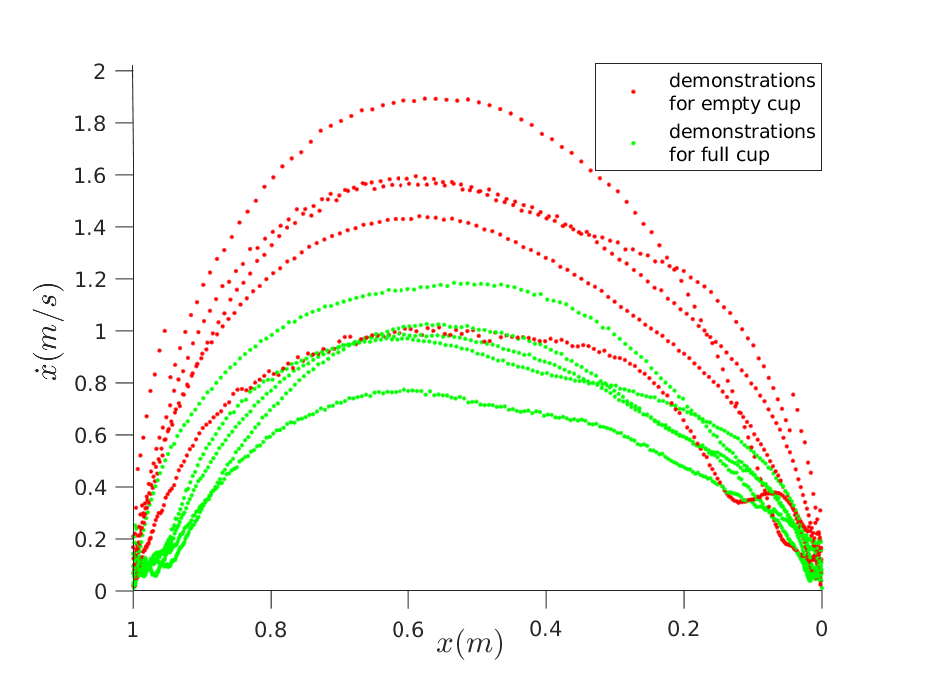
\includegraphics[width = 0.48\textwidth]{Images/vel_distance_plot.eps}
      \caption{Add legend} 
      \label{fig:vel_distance}
	\end{figure}
	
	
    \begin{figure}[t]
      \centering
      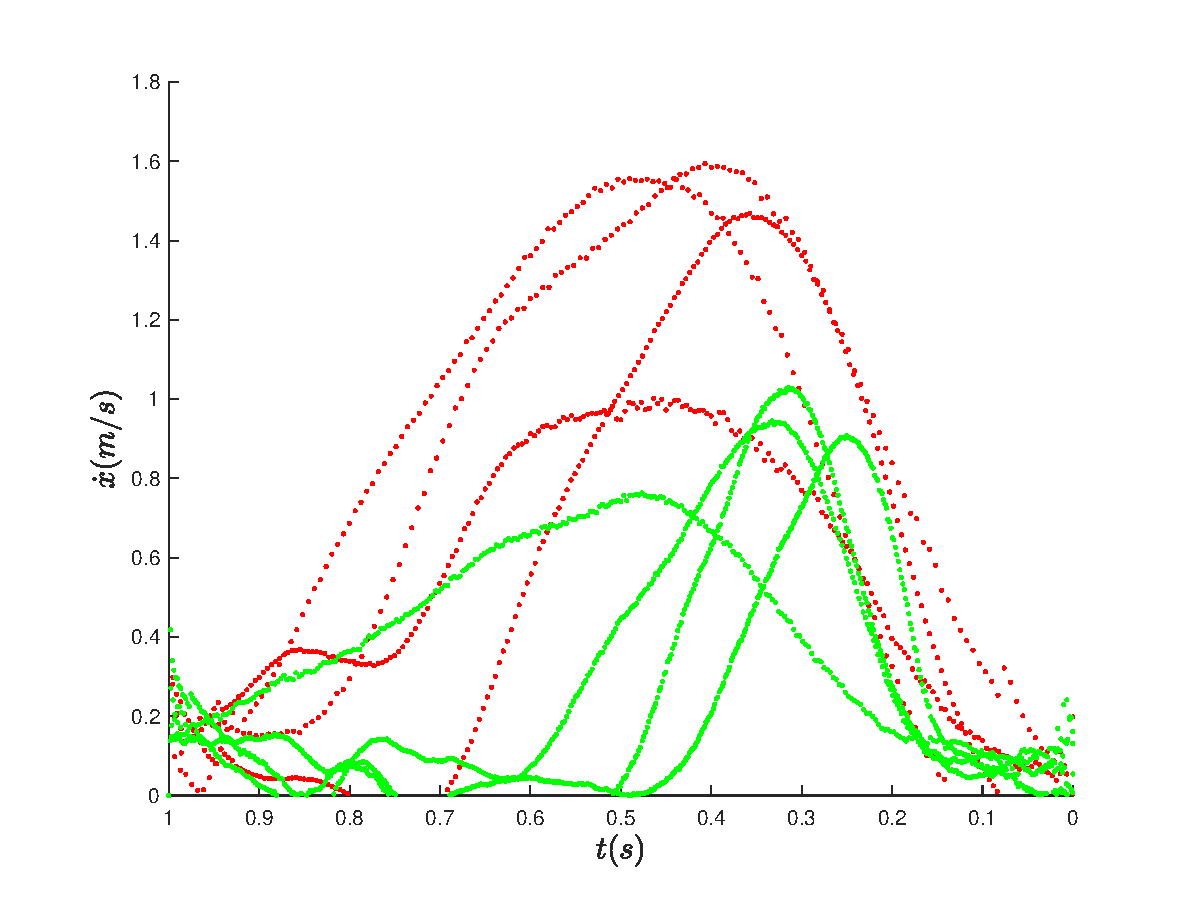
\includegraphics[width = 0.48\textwidth]{Images/vel_time_plot.eps}
      \caption{Add legend} 
      \label{fig:vel_time}
	\end{figure}
	
\section{Modelling of Handover Manipulations}

- present a short version of the deceleration phase (previous paper)
- explain why you decide to resort to this new approach
- show the results of the table of deceleration vs acceleration
- present the new approach of the acceleration phase

Let $x \in D \subset \mathbb{R}^{+}$ denote the distance of the human wrist towards the handover meeting point. Consider a behavior encoded as a state-dependent dynamical system (DS)
%
\begin{equation}
\dot{x} = \pmb{\textnormal{f}}(x)
\label{eq:1}
\end{equation}
where $\pmb{\textnormal{f}}:\mathbb{R}^{+} \to \mathbb{R}^{+}$ is a continuous and continuously differentiable function, with a single equilibrium point ${\dot{x}_d}^* = \pmb{\textnormal{f}}(x^*)$. $x^{*}$ is set at the origin and it is globally asymptotic stable such that $\dot{x}^* = \textnormal{f}(x^{*}) = 0$ which is guaranteed under a Lyapunov function $V(x):\mathbb{R}^{+} \rightarrow \mathbb{R}^{+}$.

Our approach defines each ``carefulness'' condition, \textit{careful} and \textit{not careful}, as two distinct DS. Each DS is encoded using Gaussian Mixture Models (GMM) which defines a joint distribution function $\mathcal{P}({{x}^{t}}_n, {\dot{x}^{t}}_n | \Theta) = \sum_{k=1}^{K} \pi^{k} \mathcal{N}({{x}^{t}}_n, {\dot{x}^{t}}_n, \mu^{k}, \Sigma^{k})$ over the data as mixture of $K$ Gaussian distributions \cite{khansari2011learning}, where $\pi^{k}$, $\mu^{k}$, and $\Sigma^{k}$ are, respectively, the prior component, mean, and covariance matrix of the $k$th Gaussian. $x_n^t$ is $n$th trajectory of $x$ at time $t$, and $\dot{x}_n^t$ is its derivative. Fig. \ref{fig:motion} illustrates the position ($x$) and velocity ($\dot{x}$) relations for \textit{careful} and \textit{not careful} motions. To compute the DS from Eq. (\ref{eq:1}) the posterior mean of $\mathcal{P}({\dot{x}^{t}}_n|{{x}^{t}}_n)$ is estimated which approximates it to:
%
\begin{equation}
\hat{\dot{x}} = \sum_{n=1}^{K} h^{k}(x) (\Sigma^{k}_{\dot{x}x}(\Sigma^{k}_{xx})^{-1} (x - \mu^{k}_{x}) + \mu^{k}_{\dot{x}})
\label{eq:2}
\end{equation}
where $h^{k}(x) = \frac{\pi^{k} \mathcal{N}({{x}^{t}}, {\dot{x}^{t}}, \mu^{k}, \Sigma^{k})}{\sum_{i=1}^{K} \pi^{k} \mathcal{N}({{x}^{t}}_n, {\dot{x}^{t}}_n, \mu^{i}, \Sigma^{i})}$, $h^{k}(x) > $ 0, and $\sum_{n=1}^{K} h^{k}(x)$ = 1. The GMMs are computed using the stable estimator of dynamical systems (SEDS) approach \cite{khansari2011learning}. 

  \begin{tikzpicture}
    \draw (0,3)  node[above]{Deformable}  -- (0,-3) node[below]                 {Non-deformable}(-3,0) node[xshift=-6pt,rotate=90] {Non-breakable} -- (3,0)  node[xshift=6pt,rotate=-90] {Breakable};
    \node at (-1.5,1.5) {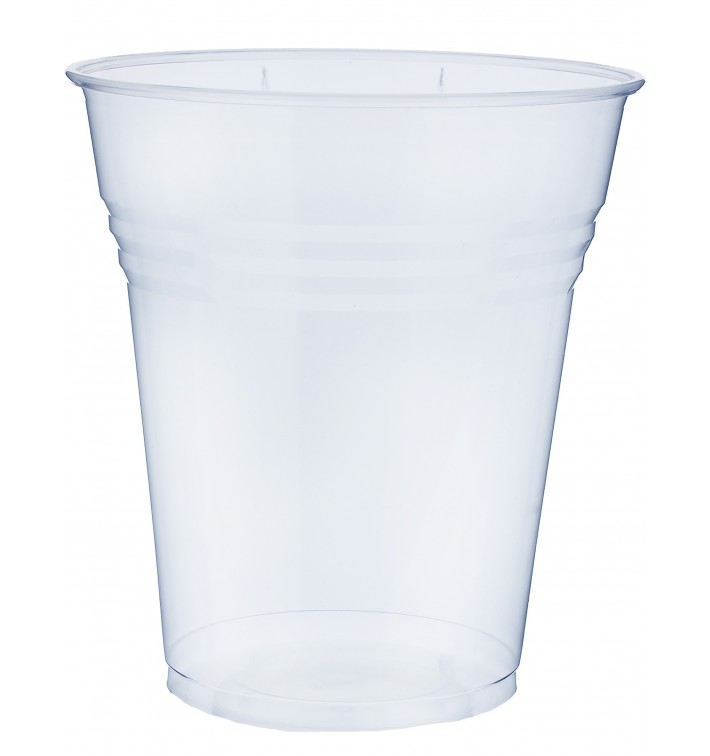
\includegraphics[width = 0.04\textwidth]{Images/transparent_cup.jpg}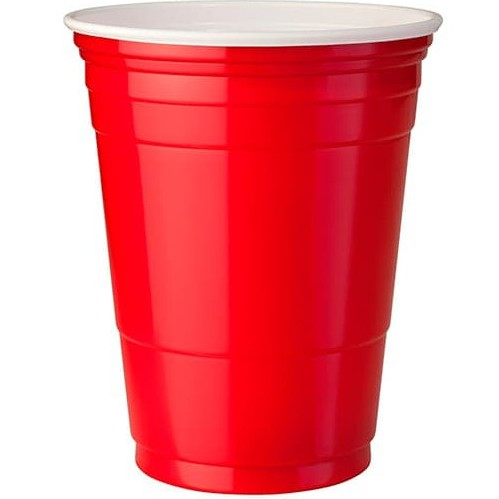
\includegraphics[width = 0.07\textwidth]{Images/red_cup.jpg}};
    \node at (1.5,1.5) {};
    \node at (-1.5,-1.5) {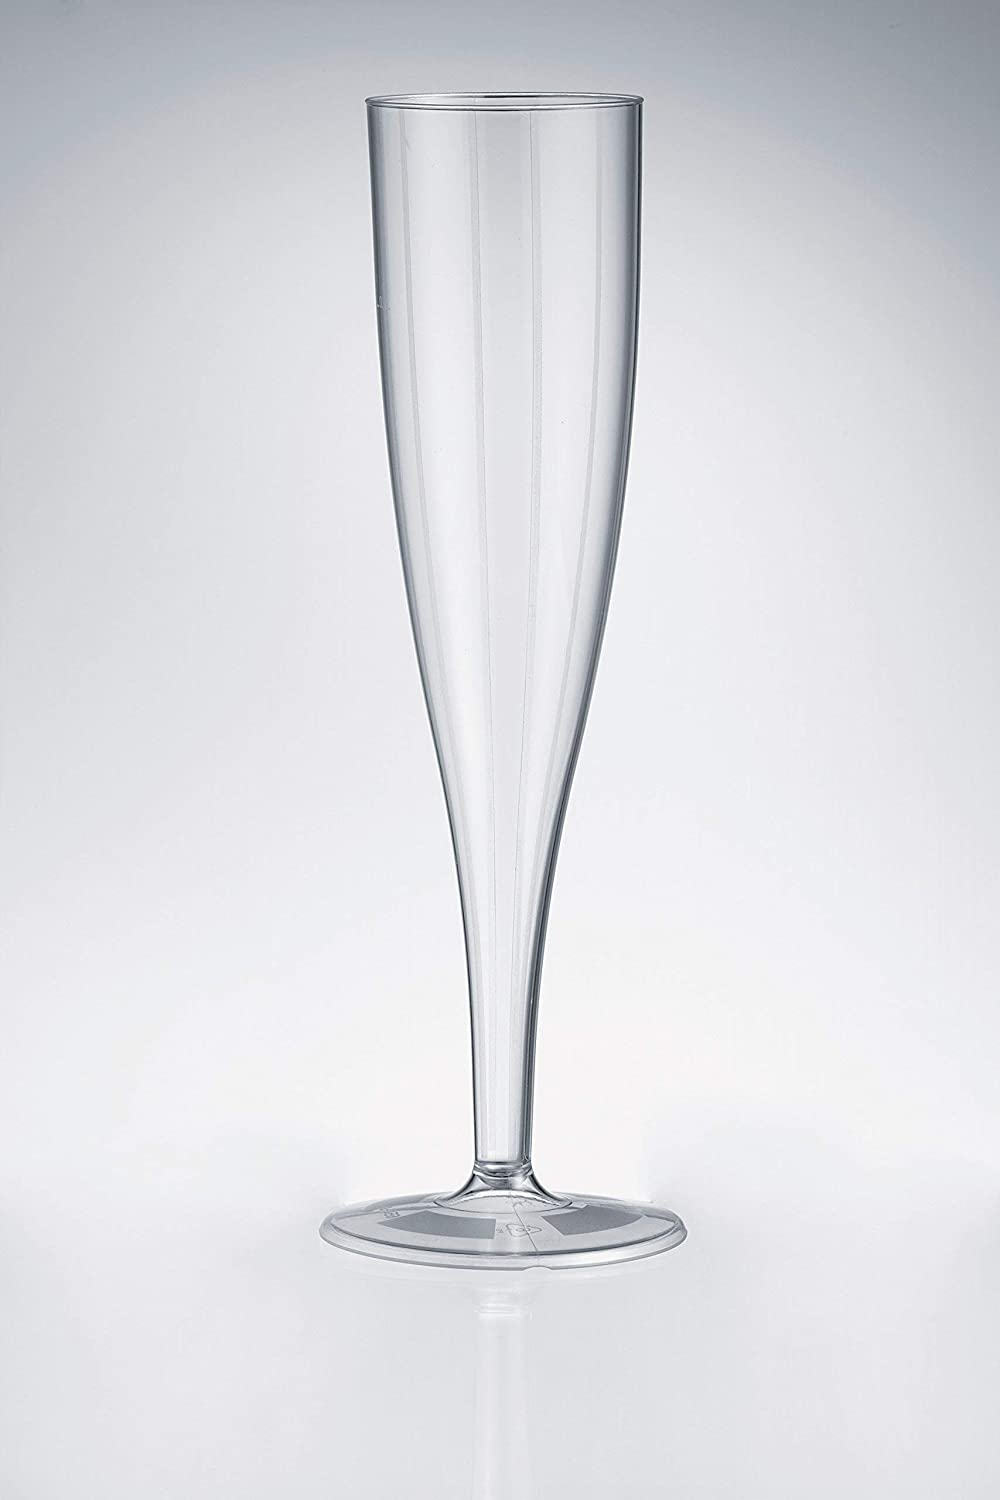
\includegraphics[width = 0.1\textwidth]{Images/champagne_cup.jpg}};
    \node at (1.5,-1.5) {
\includegraphics[width = 0.1\textwidth]{Images/wine_glass1.png}};
  \end{tikzpicture}
\section{Experimental Results}
\section{Human-Robot Applications}
\section{Conclusion}
The conclusion goes here.

% Note that keywords are not normally used for peerreview papers.
\begin{IEEEkeywords}
IEEE, IEEEtran, journal, \LaTeX, paper, template.
\end{IEEEkeywords}






% For peer review papers, you can put extra information on the cover
% page as needed:
% \ifCLASSOPTIONpeerreview
% \begin{center} \bfseries EDICS Category: 3-BBND \end{center}
% \fi
%
% For peerreview papers, this IEEEtran command inserts a page break and
% creates the second title. It will be ignored for other modes.
\IEEEpeerreviewmaketitle

% if have a single appendix:
%\appendix[Proof of the Zonklar Equations]
% or
%\appendix  % for no appendix heading
% do not use \section anymore after \appendix, only \section*
% \appendices
% \section{Proof of the First}
% you can choose not to have a title for an appendix
% if you want by leaving the argument blank
% \section{}
% Appendix two text goes here.


% use section* for acknowledgment
\section*{Acknowledgment}


The authors would like to thank...


% Can use something like this to put references on a page
% by themselves when using endfloat and the captionsoff option.
\ifCLASSOPTIONcaptionsoff
  \newpage
\fi



% trigger a \newpage just before the given reference
% number - used to balance the columns on the last page
% adjust value as needed - may need to be readjusted if
% the document is modified later
%\IEEEtriggeratref{8}
% The "triggered" command can be changed if desired:
%\IEEEtriggercmd{\enlargethispage{-5in}}

% references section

% can use a bibliography generated by BibTeX as a .bbl file
% BibTeX documentation can be easily obtained at:
% http://mirror.ctan.org/biblio/bibtex/contrib/doc/
% The IEEEtran BibTeX style support page is at:
% http://www.michaelshell.org/tex/ieeetran/bibtex/
%\bibliographystyle{IEEEtran}
% argument is your BibTeX string definitions and bibliography database(s)
%\bibliography{IEEEabrv,../bib/paper}
%
% <OR> manually copy in the resultant .bbl file
% set second argument of \begin to the number of references
% (used to reserve space for the reference number labels box)
\begin{thebibliography}{1}

\bibitem{IEEEhowto:kopka}
H.~Kopka and P.~W. Daly, \emph{A Guide to \LaTeX}, 3rd~ed.\hskip 1em plus
  0.5em minus 0.4em\relax Harlow, England: Addison-Wesley, 1999.

\end{thebibliography}

% biography section
% 
% If you have an EPS/PDF photo (graphicx package needed) extra braces are
% needed around the contents of the optional argument to biography to prevent
% the LaTeX parser from getting confused when it sees the complicated
% \includegraphics command within an optional argument. (You could create
% your own custom macro containing the \includegraphics command to make things
% simpler here.)
%\begin{IEEEbiography}[{\includegraphics[width=1in,height=1.25in,clip,keepaspectratio]{mshell}}]{Michael Shell}
% or if you just want to reserve a space for a photo:



\end{document}


